\documentclass[tikz,border=6pt]{standalone}
\usepackage{amsmath,amssymb}
\begin{document}
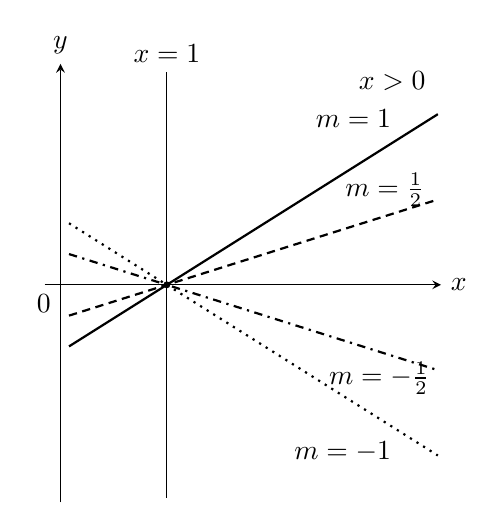
\begin{tikzpicture}[x=1.35cm,y=0.85cm,>=stealth]
  \draw[->,thin] (-0.15,0) -- (3.58,0) node[right] {$x$};
  \draw[->,thin] (0,-3.25) -- (0,3.3) node[above] {$y$};
  \node[below left] at (0,0) {$0$};

  % The group occupies the open half-plane x>0.
  \node at (3.12,3.05) {$x>0$};

  % Images y=m(x-1), together with the vertical subgroup x=1.
  \draw[thick] (0.08,-0.92) -- (3.55,2.55);
  \node[above left] at (3.2,2.2) {$m=1$};

  \draw[thick,densely dashed] (0.08,-0.46) -- (3.55,1.275);
  \node[above] at (3.05,1.03) {$m=\tfrac12$};

  \draw[thick,dash dot] (0.08,0.46) -- (3.55,-1.275);
  \node[below] at (3.0,-1.0) {$m=-\tfrac12$};

  \draw[thick,dotted] (0.08,0.92) -- (3.55,-2.55);
  \node[below left] at (3.2,-2.2) {$m=-1$};

  \draw[thin] (1,-3.18) -- (1,3.18) node[above] {$x=1$};
  \fill (1,0) circle[radius=1.25pt];
\end{tikzpicture}
\end{document}
